\documentclass[12,a4paper]{article}
\usepackage{classiccomputing}

\newcommand\postertype{lightgray}

\begin{document}

\makecclogo

\author{} % owner of the device, also used as "Author" in PDF export
\title{Mailbox / BBS}
\def\subtitle{Bulletin Board Systems}
\def\introduction{ab ca. 1980, populär bis in die späten 1990er}
\makeheader{35}{40} % title size 35, subtitle size 40

% \includeimage {images/prtel93i.png}{0.5}

\makebullets{
    Land: Weltweit \newline
    Hardware: Modems, Telefonleitungen \newline
    Platform: Jede (Atari, CP/M, Amiga, Apple, C64, DOS, OS/2, Unix, ...) \newline
    Software: Diverse BBS-Software (Server) \newline
    Software: Terminal-Programm (Client) \newline
}

\makemain{
	BBSs (Deutsch: Mailboxen) waren Computersysteme mit überwiegend textueller Benutzerschnittstelle, in
	die sich der räumlich entfernte Anwender über das Telefonnetz mittels eines Modems eingewählt hat.
	Technisch entspricht dies einem klassischen {\em seriellen Terminal}, welches aber nicht direkt über
	RS-232 an einen Computer angeschlossen wird, sondern dessen RS-232 über eine Modem-Wählverbindung
	"verlängert" wird.  \newline

	In der Zeit vor dem (für die Allgemeinheit zugänglichen) Internet boten Mailboxen die Möglichkeit des
	Austauschs von Nachrichten und Daten.  Mailboxen wurden zumeist von Privatleuten als Hobby betrieben.
	Der Betreiber wurde als {\em SysOp} (System Operator) bezeichnet.  \newline

	Es konnten nur so viele Nutzer gleichzeitig in der Mailbox eingeloggt sein, wie diese Telefonleitungen
	und Modems hatte. Dies führte zur Entwicklung von Nachrichten-Netzen auf Basis des {\em
	store-and-forward}-Prinzips, wie das FidoNet mit seiner FTN-Technik, oder Z-Netz mit
	Zerberus/ZConnect, aber auch UUCP (Unix to Unix Copy). \newline

	Auch heute gibt es noch Mailboxen, die zumeist über Telnet oder SSH im Internet erreichbar sind.  Mit
	dem Abschalten des öffentlichen PSTN- und ISDN-Netzes ist es relativ schwierig, noch echte Einwahl
	über Modems/TAs zu realisieren.
}

%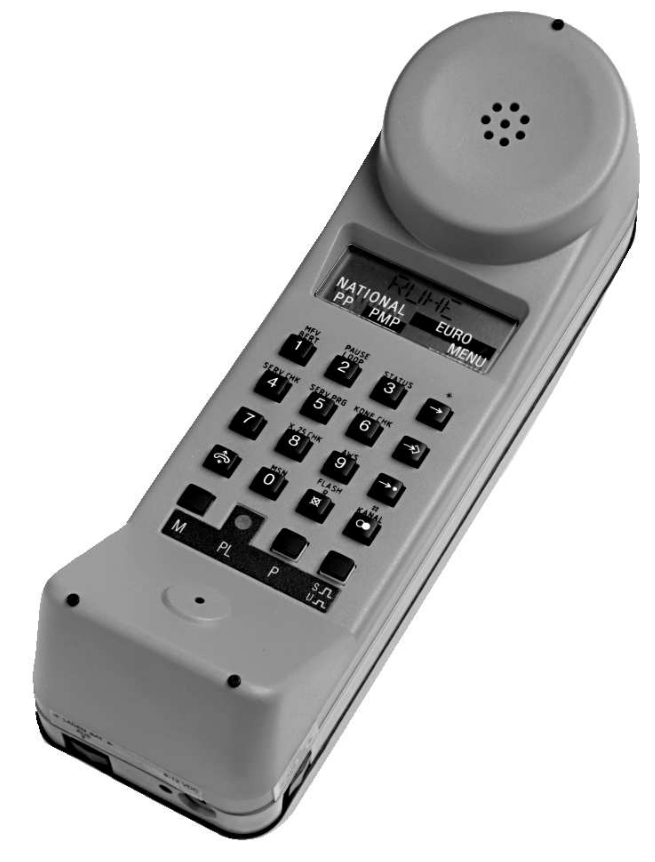
\includegraphics[width=0.5\linewidth]{images/prtel93i.png}

\makefooter

\end{document}
